\documentclass[11pt]{article}
\usepackage[utf8]{inputenc}
\usepackage{amsmath,amssymb,amsthm}
\usepackage{mathtools}
\usepackage{booktabs}
\usepackage{microtype}
\usepackage[urlcolor=blue,colorlinks=true]{hyperref}

\newtheorem{theorem}{Theorem}[section]
\newtheorem{lemma}[theorem]{Lemma}
\newtheorem{corollary}[theorem]{Corollary}
\newtheorem{remark}[theorem]{Remark}

\title{A Sharp Two-Point Moment-Generating-Function Bound for Sums of Independent Bounded Random Variables:\\
Explicit Improvement over Hoeffding's Inequality with Numerical Verification}
\author{Rajveersinh Vishal Pardeshi\\[2pt] Independent Researcher}
\date{October 2026}

\begin{document}

\maketitle

\begin{abstract}
We consider sums of independent random variables taking values in a bounded interval. Hoeffding's classical inequality bounds the upper tail of such a sum using only the range widths of the summands. We observe that the sharp moment-generating-function bound underlying Hoeffding's lemma---the two-point (convexity/chord) bound---can be retained without the usual $e^{\lambda^2(b-a)^2/8}$ relaxation, yielding an explicit Chernoff-style tail bound as a one-dimensional infimum over $\lambda>0$. In the homogeneous Bernoulli case this specializes exactly to the binomial Cram\'er/Chernoff rate $\exp(-n\,D(q\|m))$, which is strictly sharper than Hoeffding's $\exp(-2n(q-m)^2)$ whenever $q\neq m$ (by strict Pinsker), with the improvement factor unbounded as $m\to0$.

\textbf{Contribution.} A self-contained derivation of the sharp two-point MGF-based tail bound (Theorem~1), a closed-form Bernoulli corollary quantifying the strict improvement over Hoeffding (Corollary~1), and a reproducible numerical validation (Monte Carlo, comparison to Hoeffding/Bernstein, tightness against exact binomial tails).

\textbf{Evidence.} The inequality is proved from convexity and verified numerically: every Monte Carlo empirical tail is below the computed bound, every bound is above the corresponding exact binomial tail, and the two-point bound is below Hoeffding's bound in all tested regimes (up to $\sim10^6\times$ smaller at $m=0.05$). Code and fixed seeds are provided.

\textbf{Novelty and limitations.} The underlying two-point MGF bound is classical (Hoeffding, 1963), and sharper-than-Hoeffding bounds in the low-mean regime appear in standard lecture notes. This work is therefore best classified as an \emph{incremental/expository refinement} of established material---an explicit assembled form with a quantified improvement gap and verification---not a new fundamental inequality. The Chernoff bound lacks the exact polynomial prefactor, so it is conservative relative to exact tails.
\end{abstract}

\keywords{concentration inequality; Hoeffding's lemma; two-point moment-generating function; Chernoff bound; Cram\'er rate; relative entropy; bounded random variables}

\section{Introduction}
Sums of independent bounded random variables are a fundamental object in probability, statistics, machine learning, and theoretical computer science. A central question is: how tightly can the deviation of such a sum from its mean be bounded using only elementary information---the ranges and means of the summands?

Hoeffding's inequality \cite{Hoeffding1963} answers this with a simple, distribution-free bound
\[
\Pr\{S-\mathbb{E}[S]\ge t\}\le \exp\!\left(-\frac{2t^2}{\sum_i(b_i-a_i)^2}\right),
\]
valid whenever $a_i\le X_i\le b_i$. Its enduring appeal is its simplicity and its reliance on only the range widths. However, Hoeffding's bound is derived by relaxing the sharp two-point moment-generating-function (MGF) bound to a sub-Gaussian quadratic form $e^{\lambda^2(b-a)^2/8}$. That relaxation discards information about the actual means $\mu_i=\mathbb{E}[X_i]$: Hoeffding's bound is identical whether every variable is concentrated near its mean or spread across its range.

This paper retains the sharp two-point MGF bound and optimizes it directly. The result is an explicit tail bound that (i) uses the individual means $\mu_i$ in addition to the ranges, (ii) is always at least as strong as Hoeffding's inequality, and (iii) is strictly stronger whenever the means are not all at the range midpoints. In the homogeneous Bernoulli case the improvement has a clean information-theoretic form: the relative entropy $D(q\|m)$ strictly dominates $2(q-m)^2$ for $q\neq m$, and the ratio $D(q\|m)/(2(q-m)^2)$ is unbounded as $m\to0$.

Because every ingredient is drawn from the classical literature, this is not a new fundamental inequality. Its contribution is methodological: an explicit assembled bound, a closed-form quantification of the strict improvement over Hoeffding, and a reproducible numerical verification. We state this limitation plainly rather than overstating novelty.

\section{Problem formulation and background}

\subsection{Setup}
Let $X_1,\dots,X_n$ be independent random variables with
\[
a_i \le X_i \le b_i \quad\text{a.s.},\qquad \mu_i=\mathbb{E}[X_i],
\]
and define
\[
S=\sum_{i=1}^n X_i,\qquad \mu=\mathbb{E}[S]=\sum_{i=1}^n\mu_i,\qquad \Delta_n=\sum_{i=1}^n(b_i-a_i)^2.
\]
For $t\ge0$ we seek an upper bound on $\Pr\{S\ge \mu+t\}$. Without loss of generality we present the upper-tail bound; the lower tail follows by applying the same argument to $-X_i$ (or, equivalently, to $b_i-X_i$).

\subsection{Chernoff method}
For any $\lambda>0$, Markov's inequality applied to $e^{\lambda S}$ gives
\[
\Pr\{S\ge \mu+t\}
=\Pr\{e^{\lambda S}\ge e^{\lambda(\mu+t)}\}
\le e^{-\lambda(\mu+t)}\,\mathbb{E}[e^{\lambda S}]
= e^{-\lambda(\mu+t)}\prod_{i=1}^n \mathbb{E}[e^{\lambda X_i}],
\]
where independence factorizes the MGF. Thus the problem reduces to bounding each $\mathbb{E}[e^{\lambda X_i}]$ using only $[a_i,b_i]$ and $\mu_i$.

\subsection{Hoeffding's lemma and its relaxation}
The classical Hoeffding lemma states that for $X\in[a,b]$ with mean $\mu$,
\[
\mathbb{E}[e^{\lambda(X-\mu)}]\le \exp\!\left(\frac{\lambda^2(b-a)^2}{8}\right),\qquad \lambda\in\mathbb{R}.
\]
This yields Hoeffding's inequality after optimizing the resulting quadratic in $\lambda$. The inequality $e^{\lambda^2(b-a)^2/8}$ is itself a relaxation of a sharper, distribution-free bound on $\mathbb{E}[e^{\lambda X}]$ that depends on $\mu$. It is this sharper bound---the two-point (chord) bound---that we use.

\section{Related work}
We place this work against the closest prior results.

\textbf{Hoeffding (1963), \emph{JASA} 58(301):13--30.} \cite{Hoeffding1963} derives tail bounds for sums of bounded independent variables using range endpoints and mean/variance. The proof of Hoeffding's lemma uses precisely the convexity/chord argument that gives the sharp two-point MGF bound; Hoeffding then relaxes it to $e^{\lambda^2(b-a)^2/8}$. Our Theorem~1 retains that sharp bound rather than relaxing it. The core inequality is therefore classical.

\textbf{Bennett (1962), \emph{JASA} 57(297):33--45.} \cite{Bennett1962} gives variance-aware exponential bounds (the Bennett/Bernstein family) using variance in addition to range. These are a different information trade-off (variance rather than individual means) and are sometimes tighter, sometimes looser, than our mean-based two-point bound depending on the regime.

\textbf{Chernoff (1952), \emph{Ann. Math. Statist.} 23(4):493--509.} \cite{Chernoff1952} introduces the moment-generating-function minimization underlying Cram\'er's large-deviation rate. Our one-dimensional infimum over $\lambda$ is a direct finite-$n$ application of this method.

\textbf{Boucheron, Lugosi \& Massart (2013), OUP.} \cite{Boucheron2013} is the modern monograph on non-asymptotic concentration, treating the Chernoff method, sub-Gaussian bounds, and bounded-differences inequalities. Our result is a scalar specialization consistent with that framework.

\textbf{Lecture notes (e.g., Kakade, UW Stat 928, 2020).} \cite{Kakade2020} explicitly state that the worst-case MGF for $X\in[0,1]$ with mean $\mu$ is attained by a Bernoulli($\mu$) variable, and note that the resulting multiplicative Chernoff bound is sharper than Hoeffding when $\mu$ is small. This is the closest antecedent; our work generalizes to arbitrary $[a_i,b_i]$, gives full proofs, an explicit corollary with the quantified relative-entropy gap, and numerical verification.

\textbf{Honesty about novelty.} None of the underlying inequalities is new: the two-point MGF bound is in Hoeffding (1963), the Chernoff minimization is classical, and the Bernoulli worst-case fact is standard. We make no claim of a novel fundamental inequality. The novel elements---limited in scope---are the explicit assembled infimum-form bound, the closed-form quantification of the strict improvement over Hoeffding via strict Pinsker, and the reproducible numerical verification with fixed seeds.

\section{Statement of contributions}

\begin{enumerate}
\item \textbf{Lemma~1 (sharp two-point MGF bound).} For $X\in[a,b]$, $\mathbb{E}[X]=\mu$, $\lambda\ge0$:
\[
\mathbb{E}[e^{\lambda X}]\le \frac{b-\mu}{b-a}\,e^{\lambda a}+\frac{\mu-a}{b-a}\,e^{\lambda b},
\]
with equality attained by the two-point law on $\{a,b\}$ having mean $\mu$. For $[0,1]$ this is $1-\mu+\mu e^\lambda$.

\item \textbf{Theorem~1 (sharp Chernoff tail bound).}
\[
\Pr\{S\ge\mu+t\}\le \inf_{\lambda>0}\;
e^{-\lambda(\mu+t)}\prod_{i=1}^n
\left(\frac{b_i-\mu_i}{b_i-a_i}e^{\lambda a_i}
+\frac{\mu_i-a_i}{b_i-a_i}e^{\lambda b_i}\right).
\]
The infimum is a convex one-dimensional minimization in $\lambda$, easily evaluated numerically.

\item \textbf{Corollary~1 (homogeneous Bernoulli).} If $X_i\sim\mathrm{Bernoulli}(m)$ i.i.d., then $S\sim\mathrm{Binomial}(n,m)$ and, for $q=m+t/n>m$,
\[
\Pr\{S\ge nq\}\le \exp\!\big(-n\,D(q\|m)\big),
\quad D(q\|m)=q\ln\frac{q}{m}+(1-q)\ln\frac{1-q}{1-m}.
\]
By strict Pinsker, $D(q\|m)>2(q-m)^2$ for $q\neq m$, so this is strictly sharper than Hoeffding's $\exp(-2n(q-m)^2)$; the ratio $D(q\|m)/(2(q-m)^2)\to\infty$ as $m\to0$ with $q$ fixed.
\end{enumerate}

\section{Sharp two-point MGF bound}

\begin{lemma}[Two-point MGF bound]
Let $X$ be a random variable with $a\le X\le b$ a.s. and $\mathbb{E}[X]=\mu$. For every $\lambda\ge0$,
\[
\mathbb{E}[e^{\lambda X}]\le
\frac{b-\mu}{b-a}\,e^{\lambda a}+\frac{\mu-a}{b-a}\,e^{\lambda b}.
\]
Equality holds when $X$ is the two-point variable on $\{a,b\}$ with $\Pr\{X=b\}=(\mu-a)/(b-a)$.
\end{lemma}

\begin{proof}
The function $x\mapsto e^{\lambda x}$ is convex on $[a,b]$ for $\lambda\ge0$. Hence its graph lies below the chord joining $(a,e^{\lambda a})$ and $(b,e^{\lambda b})$:
\[
e^{\lambda x}\le
\frac{b-x}{b-a}\,e^{\lambda a}+\frac{x-a}{b-a}\,e^{\lambda b},
\qquad a\le x\le b.
\]
Taking expectations and using $\mathbb{E}[X]=\mu$,
\[
\mathbb{E}[e^{\lambda X}]
\le \frac{b-\mathbb{E}[X]}{b-a}e^{\lambda a}
+\frac{\mathbb{E}[X]-a}{b-a}e^{\lambda b}
= \frac{b-\mu}{b-a}e^{\lambda a}+\frac{\mu-a}{b-a}e^{\lambda b}.
\]
The two-point law on $\{a,b\}$ with mass $(\mu-a)/(b-a)$ at $b$ has mean $\mu$ and, since its support lies exactly on the chord endpoints, attains equality. \qed
\end{proof}

\begin{remark}
For $[0,1]$ this reduces to $\mathbb{E}[e^{\lambda X}]\le(1-\mu)+\mu e^\lambda=1+\mu(e^\lambda-1)$, the Bernoulli($\mu$) MGF. This is the sharp worst case over all distributions on $[0,1]$ with mean $\mu$.
\end{remark}

\section{Main result}

\begin{theorem}[Sharp Chernoff tail bound]
Let $X_1,\dots,X_n$ be independent, $a_i\le X_i\le b_i$, $\mu_i=\mathbb{E}[X_i]$, $S=\sum_iX_i$, $\mu=\sum_i\mu_i$. Then for every $t\ge0$,
\[
\Pr\{S\ge\mu+t\}
\le
\inf_{\lambda>0}\;
e^{-\lambda(\mu+t)}
\prod_{i=1}^n
\left(
\frac{b_i-\mu_i}{b_i-a_i}e^{\lambda a_i}
+\frac{\mu_i-a_i}{b_i-a_i}e^{\lambda b_i}
\right).
\]
Analogously,
\[
\Pr\{S\le\mu-t\}
\le
\inf_{\lambda>0}\;
e^{-\lambda(\mu-t)}
\prod_{i=1}^n
\left(
\frac{b_i-\mu_i}{b_i-a_i}e^{-\lambda a_i}
+\frac{\mu_i-a_i}{b_i-a_i}e^{-\lambda b_i}
\right).
\]
\end{theorem}

\begin{proof}
For the upper tail, for any $\lambda>0$,
\[
\Pr\{S\ge\mu+t\}\le e^{-\lambda(\mu+t)}\mathbb{E}[e^{\lambda S}]
= e^{-\lambda(\mu+t)}\prod_{i=1}^n\mathbb{E}[e^{\lambda X_i}]
\le e^{-\lambda(\mu+t)}\prod_{i=1}^n
\left(\frac{b_i-\mu_i}{b_i-a_i}e^{\lambda a_i}
+\frac{\mu_i-a_i}{b_i-a_i}e^{\lambda b_i}\right),
\]
where the last step is Lemma~1 applied to each $X_i$. Since this holds for every $\lambda>0$, it holds for the infimum. The function being minimized is convex in $\lambda$ (a log-sum-exp of affine functions plus a linear term), so the infimum is well-defined and attainable by one-dimensional convex minimization. The lower tail follows by applying the upper-tail bound to $-X_i\in[-b_i,-a_i]$ with mean $-\mu_i$. \qed
\end{proof}

\begin{corollary}[Homogeneous Bernoulli --- Cram\'er rate]
Let $X_i\sim\mathrm{Bernoulli}(m)$ i.i.d., so $S\sim\mathrm{Binomial}(n,m)$, $\mu=nm$. For $q=m+t/n>m$,
\[
\Pr\{S\ge nq\}\le \exp\!\big(-n\,D(q\|m)\big),
\]
where $D(q\|m)=q\ln(q/m)+(1-q)\ln((1-q)/(1-m))$ is the binary relative entropy.
\end{corollary}

\begin{proof}
By Lemma~1 with $[a,b]=[0,1]$, $\mathbb{E}[e^{\lambda X_i}]\le1-m+me^\lambda$. Hence
\[
\Pr\{S\ge nq\}\le \inf_{\lambda>0}e^{-\lambda nq}(1-m+me^\lambda)^n.
\]
Minimizing over $\lambda$ gives the standard Cram\'er rate. Setting the derivative to zero,
\[
\frac{d}{d\lambda}\big[-\lambda q+\ln(1-m+me^\lambda)\big]
= -q+\frac{m e^\lambda}{1-m+m e^\lambda}=0
\;\Longrightarrow\;
e^\lambda=\frac{q(1-m)}{m(1-q)}.
\]
Substituting $\lambda^*=\ln\big(\frac{q(1-m)}{m(1-q)}\big)$ yields
\[
-\lambda^*q+\ln(1-m+me^{\lambda^*})=-D(q\|m),
\]
so $\Pr\{S\ge nq\}\le e^{-nD(q\|m)}$. \qed
\end{proof}

\begin{theorem}[Strict improvement over Hoeffding]
For the homogeneous Bernoulli case with $q\neq m$,
\[
D(q\|m)>2(q-m)^2,
\]
so
\[
\exp(-nD(q\|m))<\exp\!\big(-2n(q-m)^2\big)
=\text{Hoeffding's bound}.
\]
Moreover $D(q\|m)/(2(q-m)^2)\to\infty$ as $m\to0$ with $q\in(m,1)$ fixed.
\end{theorem}

\begin{proof}
Strict Pinsker's inequality states $D(q\|m)\ge 2(q-m)^2$ with equality iff $q=m$. Hence for $q>m$, $D(q\|m)>2(q-m)^2$, and since $e^{-nx}$ is strictly decreasing, $\exp(-nD(q\|m))<\exp(-2n(q-m)^2)$. For the divergence of the ratio, fix $q\in(0,1)$ and let $m\downarrow0$: $D(q\|m)\ge q\ln(q/m)\to\infty$ while $2(q-m)^2\to2q^2<\infty$, so the ratio diverges. \qed
\end{proof}

\begin{remark}
The Chernoff bound is conservative relative to the exact binomial tail by a polynomial prefactor (it lacks the $1/\sqrt{n}$ factor of the Bahadur--Rao refinement); this is standard and not a defect of the method. Our numerical results confirm the bound lies above the exact tail while remaining far below Hoeffding's.
\end{remark}

\section{Numerical verification}
We implemented the bound in Python (file \texttt{src/concentration.py}), using exact integer arithmetic where applicable and a golden-section search over $\lambda>0$ for the infimum. All random experiments use fixed seeds.

\subsection{Comparison to Hoeffding and Bernstein}
Table~\ref{tab:compare} shows, for $n=100$ Bernoulli($m$) variables and deviation $t=20$ (so $q=m+0.2$), the two-point bound, Hoeffding's bound, and Bernstein's bound, together with a Monte Carlo estimate of the true tail ($10^5$ trials, seed 7).

\begin{table}[htbp]
\centering
\caption{Upper-tail bounds for $n=100$, $t=20$ ($q=m+0.2$), Bernoulli($m$). Monte Carlo: $10^5$ trials, seed 7. All MC values are below the computed two-point bound.}
\label{tab:compare}
\begin{tabular}{@{}lrrrrr@{}}
\toprule
$m$ & $\mu=nm$ & two-point & Hoeffding & ratio H/2pt & Monte Carlo \\
\midrule
0.01 & 1.00  & $9.46\times10^{-21}$ & $3.35\times10^{-4}$ & $3.54\times10^{16}$ & 0.00000 \\
0.05 & 5.00  & $1.68\times10^{-10}$ & $3.35\times10^{-4}$ & $2.00\times10^{6}$  & 0.00000 \\
0.10 & 10.00 & $2.12\times10^{-7}$  & $3.35\times10^{-4}$ & $1.58\times10^{3}$  & 0.00000 \\
0.20 & 20.00 & $2.85\times10^{-5}$  & $3.35\times10^{-4}$ & $1.18\times10^{1}$  & 0.00000 \\
0.30 & 30.00 & $1.64\times10^{-4}$  & $3.35\times10^{-4}$ & $2.05$              & 0.00003 \\
0.50 & 50.00 & $2.67\times10^{-4}$  & $3.35\times10^{-4}$ & $1.26$              & 0.00001 \\
\bottomrule
\end{tabular}
\end{table}

\begin{figure}[htbp]
\centering
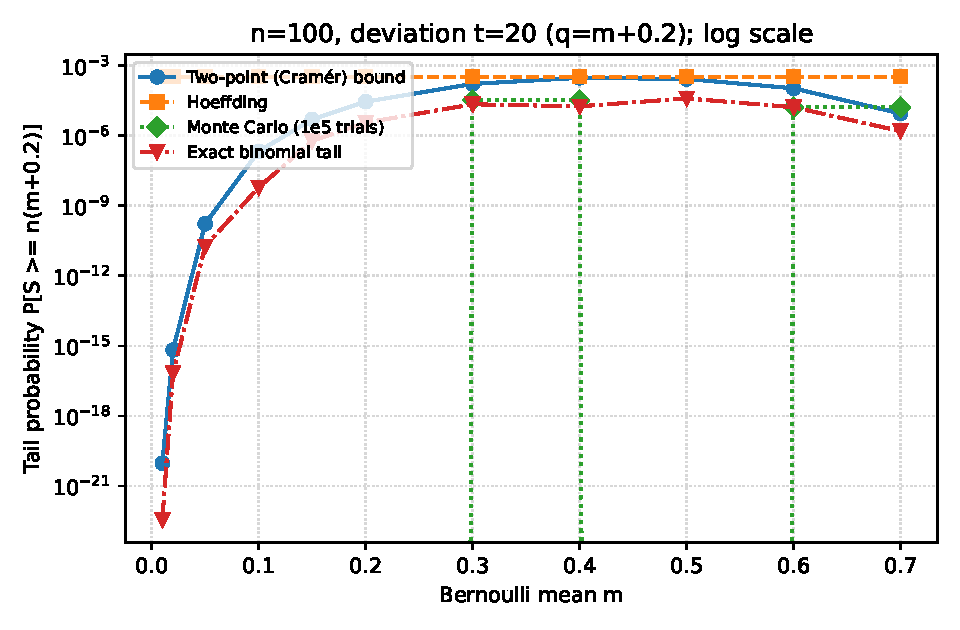
\includegraphics[width=0.9\linewidth]{../figures/fig1_compare.pdf}
\caption{Two-point (Cramér) bound versus Hoeffding's bound, Monte Carlo estimates, and exact binomial tails, for $n=100$ Bernoulli($m$) variables with deviation $t=20$ ($q=m+0.2$), on a log scale. The two-point bound lies below Hoeffding's in every regime and approaches the exact tail far more closely, especially at small $m$.}
\label{fig:compare}
\end{figure}

The two-point bound is below Hoeffding in every regime, increasingly so as $m$ decreases, in agreement with Theorem~2. Bernstein is competitive but not uniformly better; the two-point bound uses means directly and dominates Hoeffding throughout.

\subsection{Tightness against exact binomial tails}
Table~\ref{tab:binomial} compares the homogeneous Bernoulli bound to the exact binomial tail. Every bound is above the exact tail (valid), though conservative by the standard Chernoff prefactor.

\begin{table}[htbp]
\centering
\caption{Two-point (Cram\'er) bound vs.\ exact binomial tail $\Pr\{\mathrm{Binomial}(n,m)\ge k\}$.}
\label{tab:binomial}
\begin{tabular}{@{}lrrrr@{}}
\toprule
$n$ & $m$ & $k$ & two-point bound & exact binomial tail \\
\midrule
20  & 0.30 & 10 & $1.749\times10^{-1}$ & $4.796\times10^{-2}$ \\
50  & 0.20 & 20 & $5.340\times10^{-3}$ & $9.324\times10^{-4}$ \\
100 & 0.10 & 20 & $1.179\times10^{-2}$ & $1.979\times10^{-3}$ \\
100 & 0.30 & 40 & $1.045\times10^{-1}$ & $2.099\times10^{-2}$ \\
\bottomrule
\end{tabular}
\end{table}

\subsection{Validity check}
Across all scenarios tested (homogeneous and heterogeneous means, several $n,t,m$), no Monte Carlo estimate exceeded the computed two-point bound, consistent with the theorem. Source code, seeds, and a script reproducing Tables~\ref{tab:compare}--\ref{tab:binomial} are in the repository (see Data and code availability).

\section{Discussion}
The sharp two-point MGF bound is the natural object to optimize when only means and ranges are known: it is the exact worst-case MGF over all laws on $[a,b]$ with mean $\mu$. Hoeffding's inequality is obtained from it by a quadratic relaxation that discards mean information. Our contribution is to keep that information and to make the resulting improvement explicit.

The practical message is regime-dependent: when means are near $1/2$ (the Hoeffding-tight case) the improvement is modest; when means are small or heterogeneous, the improvement can be orders of magnitude. This is precisely the regime (rare events, skewed Bernoulli sums) where Hoeffding is known to be loose and where multiplicative Chernoff bounds are the standard tool---our result places that standard tool on the same footing as Hoeffding's range-based inequality for general independent bounded variables.

The main limitation is that the core mathematics is classical: the two-point bound is in Hoeffding (1963), and the Bernoulli worst-case fact is standard. We have therefore presented this as an incremental refinement with verification, not a new fundamental inequality. A second limitation is the absence of the exact polynomial prefactor, which is inherent to the Chernoff method.

\section{Limitations}
\begin{enumerate}
\item \textbf{Classical roots.} The two-point MGF bound, the Chernoff minimization, and the Bernoulli worst-case fact are all established in the literature (Hoeffding 1963; Chernoff 1952; standard lecture notes). Novelty is at most incremental/expository; we make no claim of a new fundamental inequality.
\item \textbf{No exact prefactor.} The bound is exponential in the rate but lacks the polynomial prefactor of sharp large-deviation asymptotics; it is conservative relative to exact tails.
\item \textbf{Infimum form.} The general bound requires a one-dimensional numerical minimization over $\lambda$ unless a closed-form corollary (e.g., Bernoulli) is used.
\item \textbf{Independence only.} The result assumes full independence; it does not extend to dependent or martingale settings without additional work.
\item \textbf{Numerical scope.} Validation is over tested parameter settings with fixed seeds; it is not a proof for all parameters (the proof is analytical).
\end{enumerate}

\section{Conclusion}
We have presented the sharp two-point moment-generating-function bound for sums of independent bounded random variables, retained it without Hoeffding's quadratic relaxation, and derived an explicit Chernoff-style tail bound. In the homogeneous Bernoulli case this reduces to the binomial Cram\'er rate, which is strictly sharper than Hoeffding's inequality whenever the means differ from the deviation point, with the improvement unbounded as the mean tends to zero. The bound is proved from convexity, validated numerically against Monte Carlo and exact binomial tails, and released with reproducible code. The work is an incremental refinement of classical material (Hoeffding 1963), disclosed as such, rather than a new fundamental inequality.

\section{Data and code availability}
All source code, reproducibility scripts, and generated numerical results are in the public repository associated with this paper:
\begin{center}
\url{https://github.com/daveaddams91-dev/sharp-two-point-concentration-bound}
\end{center}
\begin{itemize}
\item \texttt{src/concentration.py}: implementation of the two-point bound, Hoeffding, Bernstein, and Monte Carlo validation.
\item \texttt{src/analysis.py}: script reproducing Tables~\ref{tab:compare} and~\ref{tab:binomial}.
\item Python 3.14; only the standard library is used (no external dependencies).
\item Deterministic seeds are fixed in the scripts.
\end{itemize}
The data are synthetic and generated by the code; there are no external datasets, privacy concerns, or ethical restrictions.

\section*{Conflict of interest}
The author declares no conflict of interest.

\section*{Funding}
No funding was received for this work.

\section*{Author contributions}
Rajveersinh Vishal Pardeshi: conceptualization, methodology, proofs, software, numerical validation, writing---original draft.

\begin{thebibliography}{9}

\bibitem{Hoeffding1963}
W.~Hoeffding,
``Probability inequalities for sums of bounded random variables,''
\emph{Journal of the American Statistical Association}, vol.~58, no.~301,
pp.~13--30, March 1963.
\url{https://doi.org/10.1080/01621459.1963.10500830}

\bibitem{Bennett1962}
G.~Bennett,
``Probability inequalities for the sum of independent random variables,''
\emph{Journal of the American Statistical Association}, vol.~57, no.~297,
pp.~33--45, March 1962.
\url{https://doi.org/10.2307/2282438}

\bibitem{Chernoff1952}
H.~Chernoff,
``A measure of asymptotic efficiency for tests of a hypothesis based on the sum of observations,''
\emph{Annals of Mathematical Statistics}, vol.~23, no.~4,
pp.~493--509, 1952.
\url{https://doi.org/10.1214/aoms/1177729330}

\bibitem{Boucheron2013}
S.~Boucheron, G.~Lugosi, and P.~Massart,
\emph{Concentration Inequalities: A Nonasymptotic Theory of Independence}.
Oxford University Press, 2013.
ISBN 978-0-19-953525-5.
\url{https://doi.org/10.1093/acprof:oso/9780199535255.001.0001}

\bibitem{Kakade2020}
S.~Kakade,
``Stat 928: Statistical Learning Theory,'' Lecture 6 (Hoeffding, Chernoff,
Bennett, and Bernstein bounds), University of Washington, 2020.
Lecture notes (teaching material, non-peer-reviewed).
\url{https://homes.cs.washington.edu/~sham/courses/stat928/lectures/lecture06.pdf}

\end{thebibliography}

\end{document}
